\documentclass{article}
\usepackage[utf8]{inputenc}
\usepackage{amsmath}
\usepackage{tcolorbox}
\usepackage{indentfirst}
\usepackage{graphicx}
\usepackage{minted}
\usepackage{float}
\usepackage [english]{babel}
\usepackage [autostyle, english = american]{csquotes}
\MakeOuterQuote{"}

\title{System on a Chip Class Report 3}
\author{Jordan D Edwards}
\date{October 2023}


\begin{document}
	
	\title{Class Report 4
		\\ \large{ELC 4396 System on a Chip}  }
	
	\author{Jordan Edwards \\ Baylor University} %the \\ symbols starts a new line
	\date{November 2, 2023}
	\maketitle
	
	\subsection*{Introduction}
	For this assignment, I added SPI functionality to my system and demonstrated its functionality by building a small demo with the built-in accelerometer and seven-segment displays.
	
	
	\subsection*{Implementation}
	In Vivado, I added the necessary components to the MMIO bridge and routed all of the communication wires through to the top level of the project. I was then able to export the bit file in order to continue working on the project in Vitis. Once in Vitis, I opened the example files to understand the exact commands that the accelerometer was expecting. With this information, I modified his function in order to return my own data type, a Vector3. This data type allowed me to easily access all three components of the acceleration data as well as normalize the result in order to get a simple unit vector in the direction of "up." I used this to simply decide whether the X or Y component was larger, and then I used that information to light up a single edge of a single digit of the seven-segment display.
	
	\begin{figure}[H]
		\centering
		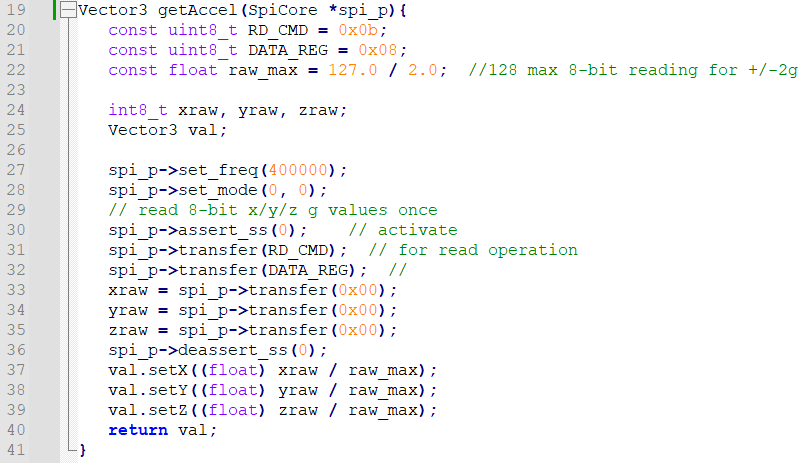
\includegraphics[width=\linewidth]{getAccel}
		\caption{Get acceleration function}
		\label{fig:func}
	\end{figure}
	
	
	\begin{figure}[H]
		\centering
		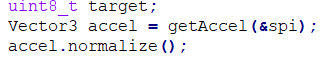
\includegraphics[width=.6\linewidth]{functionCall}
		\caption{Simple fetch and normalization with Vector3}
		\label{fig:call}
	\end{figure}
	
	\begin{figure}[H]
		\centering
		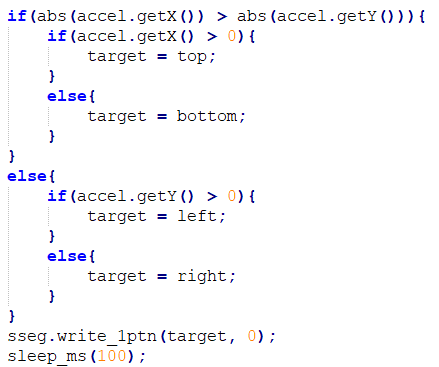
\includegraphics[width=.75\linewidth]{display}
		\caption{Directionality tests}
		\label{fig:disp}
	\end{figure}

	
	\subsection*{Results}
	The code ran successfully on the board; when tilted, the correct segments on the seven-segment display were illuminated. Because there is no filtering and only accelerometer data is used, shaking the board can cause the display to change rapidly even if it is tilted at a steep angle.
\end{document}
